\documentclass[10pt, letterpaper]{article}
\usepackage{geometry}
\geometry{
 a4paper,
 total={170mm,257mm},
 left=20mm,
 top=20mm,
 }
\usepackage{graphicx} % Required for inserting images
\usepackage[english,greek]{babel}
\usepackage{amsmath} 
\usepackage{subcaption}
\usepackage{dirtytalk}
\usepackage{multirow}
\usepackage{hyperref}
\usepackage{comment}
\usepackage{tikz}
\usepackage{caption}
\usepackage{float}
\usepackage{amssymb}
\usepackage{indentfirst}
\newcommand{\en}{\selectlanguage{english}}
\newcommand{\gr}{\selectlanguage{greek}}


\graphicspath{{../plots/}} % specify the path to the images

\title{Εργασία Υπολογιστικού Ηλεκτρομαγνητισμού}
\author{Φίλιππος Ρωσσίδης \\ (ΑΕΜ 10379)}
\date{\today}


\begin{document}
\maketitle
\begin{comment}
  

\section*{Μέρος Α}

Στο πρώτο μέρος της εργασίας θα χρησιμοποιήσουμε την μέθοδο \en FEM \gr για να επιλύσουμε δύο ηλεκτροστατικά προβλήματα: ενός ομοαξονικού καλωδίου 
(σχήμα \ref{fig:coaxial}) όπου ο εσωτερικός αγωγός τίθεται σε δυναμικό 1 \en Volt \gr και ο εξωτερικός σε 0 \en Volt, \gr 
και ενός πυκνωτή απείρου μήκους, με διαστάσεις που φαίνονται στο σχήμα \ref{fig:capacitor} και διαφορά δυναμικού \en V. \gr

Θα χρησιμοποιήσουμε την μέθοδο \en FEM \gr για την εύρεση του δυναμικού στο χώρο και έπειτα απο το δυναμικό θα υπολογίσουμε 
το ηλεκτρικό πεδίο, την ενέργεια και την χωρητικότητα. 


\begin{figure}[H]
    \centering
    % Subfigure (a): Ομοαξονικό
    \begin{subfigure}[b]{0.45\textwidth}
      \centering
      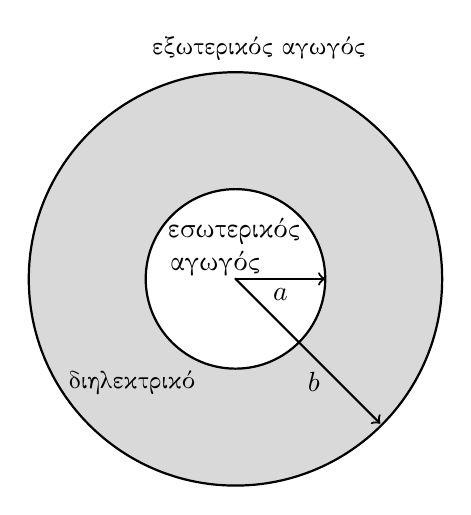
\begin{tikzpicture}[scale=1.5]
        % Radii
        \def\a{0.76}
        \def\b{1.75}
      
        % Annular dielectric region (from a to b)
        \fill[gray!30] (0,0) circle (\b);
        \fill[white] (0,0) circle (\a); % Inner conductor kept white
      
        % Outer conductor
        \draw[thick] (0,0) circle (\b);
      
        % Inner conductor (white-filled with border)
        \draw[thick] (0,0) circle (\a);
      
        % Radius a (along x-axis)
        \draw[->, thick] (0,0) -- (\a,0);
        \node[below] at (\a/2, 0) {\( a \)};
      
        % Radius b (along diagonal)
        \draw[->, thick] (0,0) -- (1.4 /2 * \b ,- 1.4 / 2* \b);
        \node[left] at (\b/2.2, -\b/2) {\( b \)};
      
        % Center point
        \fill (0,0) circle (0.01);
      
        % Labels
        \node[align=center, text width=1.2cm] at (-0.17, \a - 0.5) {εσωτερικός\\αγωγός};
        \node at (0.2, \b + 0.2) {\small εξωτερικός αγωγός};
        \node at (-\b/2, -\b/2) {\small διηλεκτρικό};
      \end{tikzpicture}
      \caption{Ομοαξονικό καλώδιο}
      \label{fig:coaxial}
    \end{subfigure}
    \hfill
    % Subfigure (b): Πυκνωτής
    \begin{subfigure}[b]{0.45\textwidth}
        \centering
        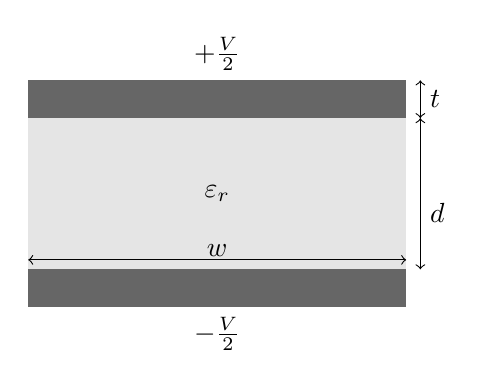
\begin{tikzpicture}[scale=1.2]
        \def\d{2}   % Απόσταση μεταξύ πλακών
        \def\w{4}   % Πλάτος πλακών
        \def\t{0.4}   % Πάχος πλακών
    
        % Κάτω πλάκα (με λίγο κενό κάτω για να χωρέσει η διάσταση w)
        \fill[black!60] (-\w/2, 0.3) rectangle (\w/2, 0.3+\t);
        \node[below] at (0, 0.3) {\( -\frac{V}{2} \)};
    
        % Πάνω πλάκα
        \fill[black!60] (-\w/2, 0.3+\d) rectangle (\w/2, 0.3+\d+\t);
        \node[above] at (0, 0.3+\d+\t) {\( +\frac{V}{2} \)};
    
        % Διηλεκτρικό
        \fill[gray!20] (-\w/2, 0.3+\t) rectangle (\w/2, 0.3+\d);
    
        % Διαστάσεις
        % Απόσταση d
        \draw[<->] (\w/2 + 0.15, 0.3+\t) -- (\w/2 + 0.15, 0.3+\d);
        \node[right] at (\w/2 + 0.15, 0.3+\d/2) {\( d \)};
        
        % Πλάτος w
        \draw[<->] (-\w/2, 2* \t) -- (\w/2, 2 * \t);
        \node at (0, 2 * \t + 0.1) {\( w \)};
    
        % Πάχος t (πάνω πλάκας)
        \draw[<->] (\w/2 + 0.15, 0.3+\d) -- (\w/2 + 0.15, 0.3+\d+\t);
        \node[right] at (\w/2 + 0.15, 0.3+\d+\t/2) {\( t \)};
    
        % Διηλεκτρική σταθερά στο κέντρο
        \node at (0, 0.5+\d/2) {\( \varepsilon_r \)};
        \end{tikzpicture}
        \caption{Πυκνωτής παράλληλων πλακών}
        \label{fig:capacitor}
    \end{subfigure}
    \caption{}
    \label{fig:definition}
  \end{figure}


\subsection*{Σύντομη περιγραφή της μεθόδου \en FEM \gr για την εύρεση δυναμικού σε ηλεκτροστατικό πρόβλημα}

Θα παρουσιάσω σύντομα την μέθοδο, για την πληρότητα της αναφοράς. Σε κάποια σημεία χρησιμοποιώ διαφορετικό 
συμβολισμό από τις σημειώσεις γιατι το θεώρησα πιο ευανάγνωστο.

Αρχικά, εφόσον λύνουμε δισδιάστατα προβλήματα, χωρίζουμε τον υπολογιστικό χώρο σε \en 2d simplexes \gr δηλαδή τρίγωνα. 
Αν οριστούν οι συντεταγμένες \en simplex \gr ενός σημείου $(x,y)$ ως $\zeta_i(x,y) = h_i / H_i$ όπου $h_i$ η απόσταση του σημείου 
από την πλευρά που δεν περιέχει τον κόμβο $i$ και $H_i$ το ύψος από τον κόμβο $i$, τότε 
\[ \zeta_i(x,y) = a_i + b_ix + c_iy, \ \ i = 1,2,3 \]
όπου τα $a_i,b_i,c_i$ δίνονται με κυκλική εναλλαγή απο τις:
\begin{equation} \label{eq:abc}
  a_1 = \frac{x_2 y_3 - x_3 y_2}{D}, \quad
b_1 = \frac{y_2 - y_3}{D}, \quad
c_1 = \frac{x_3 - x_2}{D},
\end{equation}
\[ D =  
\left| 
\begin{array}{@{}ccc@{}}
1 & x_1 & y_1 \\
1 & x_2 & y_2 \\
1 & x_3 & y_3 \\
\end{array} 
\right|
\]
Αναλύουμε, εντός του τριγώνου, το δυναμικό ως 
\[ \phi \approx \sum_{i=1}^3 \phi_iN_i^t\]
όπου $\phi_i$ το δυναμικό στον κόμβο $i$ και διαλέγουμε $N_i^t=\zeta_i$ τις τοπικές (εντός του τριγώνου $t$) συναρτήσεις βάσης.
Σκοπός μας είναι να βρούμε τις κατάλληλες τιμές $\phi_i$ για κάθε κόμβο στον υπολογιστικό χώρο.
Έτσι ορίζουμε τις ολικές συναρτήσεις βάσης ως 
\[ N_p = \sum_{t | p \in t} N_i^t \]
όπου $t$ τρίγωνο τέτοιο ώστε ο κόμβος $p$ να ανήκει σε αυτό, και $i$ η τοπική αρίθμηση του $p$ στο $t$.
Το δυναμικό αναλύεται συνολικά:
\begin{equation} \label{eq:phi_approx}
  \phi \approx \sum_{p=1}^{N_n} \phi_pN_p
\end{equation}
όπου $N_n$ το πλήθος κόμβων.
Θα λύσουμε την εξίσωση \en Poisson: \gr 
\[ \nabla \cdot (\epsilon \nabla \phi) + \rho = 0\]
χρησιμοποιώντας την μέθοδο \en Galerkin \gr η οποία αποτελεί κατηγορία της μεθόδου σταθμισμένων υπολοίπων:
\[ \langle \phi', \nabla \cdot (\epsilon \nabla \phi) + \rho \rangle = 0 \]
όπου διαλέγουμε ως συναρτήσεις 
δοκιμής $\phi'$ τις συναρτήσεις βάσης $N_i$, οπότε:
\[ \iint_{\Omega} \phi' [ \nabla \cdot (\epsilon \nabla \phi) + \rho ] ds = 0, \ \ \forall \phi' \in \{N_i\} \]
όπου $\Omega$ ο υπολογιστικός χώρος. 
Οι παραπάνω είναι τόσες εξισώσεις όσους έχουμε άγνωστους κόμβους, τους οποίους θα βρούμε λύνοντας το σύστημα.
Ισοδύναμα γράφονται:
\begin{equation} \label{eq:weak_form}
  -\iint_{\Omega} \nabla \phi' \cdot \epsilon \nabla \phi ds +  \oint_{c} \phi' \epsilon \frac{\partial \phi}{\partial \hat{n}}dl + \iint_{\Omega} \phi' \rho ds = 0
\end{equation}
όπου $c$ το όριο της επιφάνειας $\Omega$. 

Αν έχουμε ομογενής συνθήκες \en Neumann \gr 
($\frac{\partial \phi}{\partial \hat{n}} = 0$) ο δεύτερος όρος της εξίσωσης (\ref{eq:weak_form}) ισούται με 0.
Επίσης αν έχουμε συνθήκες \en Dirichlet \gr (γνωστό $\phi$) οι συναρτήσεις 
δοκιμής $\phi' \in {N_i}$ θα είναι 0 στο όριο (οι κόμβοι που ανήκουν 
στο όριο είναι γνωστοί και δεν έχουν συνάρτηση βάσης).
Θεωρούμε ότι δεν έχουμε άλλου είδους οριακές συνθήκες. Έτσι
ο δεύτερος όρος της εξίσωσης (\ref{eq:weak_form}) ισούται με 0. Επίσης και στα δύο προβλήματα 
δεν υπάρχουν φορτία ($\rho = 0$), άρα:
\[ \iint_{\Omega} \nabla \phi' \cdot \epsilon \nabla \phi ds = 0\]
Διακριτοποιώ αντικαθιστώντας την εξίσωση (\ref{eq:phi_approx}), επίσης αφού $\phi' \in \{N_i\}$ γράφω στη θέση του $N_q$ για κάποιο $q \in \{1,..,N_n\}$:
\[ \iint_{\Omega} \nabla N_q(\mathbf{r}) \cdot \epsilon \nabla (\sum_p \phi_p N_p(\mathbf{r}))  ds = 0 \Rightarrow\]
\begin{equation} \label{eq:sum_out}
  \sum_p  \phi_p \iint_{\Omega} \nabla N_q(\mathbf{r}) \cdot \epsilon \nabla N_p(\mathbf{r})ds = 0
\end{equation}

Ισχύει:
\[ N_i^t (x,y) =  \zeta_i(x,y) = a_i + b_ix + c_iy, \text{\ εντός του στοιχείου και $0$ αλλού}\Rightarrow\]
\[ \nabla N_i^t =   
    \begin{bmatrix}
        b_i \\
        c_i
    \end{bmatrix}
                    , \text{\ εντός του στοιχείου και $0$ αλλού}\]
Για κάθε κόμβο η ολική συνάρτηση βάσης εντός κάθε τριγώνου στο οποίο αυτός ανήκει ισούται με 
την τοπική συνάρτηση βάσης του σε αυτό το τρίγωνο και εκτός αυτών με μηδέν.
Έπεται ότι το γινόμενο $\nabla N_p \cdot \epsilon \nabla N_q$ ισούται με $0$ για μη γειτονικούς κόμβους. Για γειτονικούς κόμβους $p,q$ όπου 
ανήκουν και οι δύο σε κάποιο 
τρίγωνο $t$, ισχύει εντός του τριγώνου
\[ \nabla N_p  \cdot \epsilon \nabla N_q  = \nabla N_i^t \cdot \epsilon \nabla N_j^t = 
    \begin{bmatrix}
        b_i \\
        c_i
    \end{bmatrix}
      \cdot \epsilon
    \begin{bmatrix}
        b_j \\
        c_j        
    \end{bmatrix}
    =  \epsilon (b_ib_j + c_ic_j)
\]
με $i,j$ την τοπική αρίθμηση εντός του $t$. Έτσι, θεωρώντας ότι το $\epsilon$ είναι σταθερό εντός κάθε στοιχείου:
\begin{equation} \label{eq:int_of_grad_Np_Nq_}
  \iint_S \nabla N_p  \cdot \epsilon \nabla N_q  dS = \sum_{t | p,q \in t} \epsilon (b_ib_j + c_ic_j) A_e 
\end{equation}
δηλαδή άθροισμα της ποσότητας $(b_ib_j + c_ic_j) A_e $ για κάθε τρίγωνο $t$ που περιέχει και τον $p$ και τον $q$, 
όπου $i,j$ η τοπική αρίθμηση των κόμβων $p,q$ στο τρίγωνο $t$, οι $b,c$ δίνονται από την (\ref{eq:abc}) και $A_e = D/2$ το εμβαδόν του τριγώνου.
Η (\ref{eq:sum_out}) γράφεται:
\begin{equation}  \label{eq:system_non_matrix_form}
  \sum_p  \phi_p \sum_{t | p,q \in t} \epsilon (b_ib_j + c_ic_j) A_e  = 0   \ \ \forall q \in \{1,..,N_n\}
\end{equation}
Αν ορίσω τον τετραγωνικό πίνακα $N_n \times N_n$ $\mathbf{S}$:
\[ \mathbf{S}[p,q] =  \sum_{t | p,q \in t} \epsilon (b_ib_j + c_ic_j) A_e  \]
και τον πίνακα στήλη $1 \times N_n$ $\mathbf{F}$ που περιέχει τα δυναμικά των κόμβων $\phi_p$, τότε το σύστημα (\ref{eq:system_non_matrix_form}) γράφεται:
\[ \mathbf{S} \cdot \mathbf{F} = \mathbf{0} \]

Μπορούμε να υπολογίσουμε εύκολα τον πίνακα $\mathbf{S}$ αν απαριθμήσουμε κάθε τρίγωνο στον χώρο και έπειτα για κάθε έναν από τους
9 συνδυασμούς των κόμβων του (έστω $p,q$ ολικά, $i,j$ τοπικά) υπολογίσουμε την ποσότητα $\epsilon (b_ib_j + c_ic_j) A_e$ και την προσθέσουμε στην θέση $[p,q]$ του πίνακα.

Τέλος πρέπει να λάβουμε υπόψη τους κόμβους με οριακή συνθήκη \en Dirichlet \gr δηλαδή γνωστού δυναμικού. Επειδή ο πίνακας $\mathbf{F}$ είναι η λύση,
δεν μπορεί να περιλαμβάνει τα γνωστά δυναμικά, έτσι τον χωρίζουμε τοποθετώντας πρώτα τα άγνωστα και έπειτα τα γνωστά:

\[
\mathbf{F} = 
\left[ \begin{array}{@{}c@{}}
\mathbf{F}_f \\
\hline
\mathbf{F}_p
\end{array} \right]
, \ \
\mathbf{S} = 
\left[ \begin{array}{@{}c|c@{}}
  \mathbf{S}_{ff} & \mathbf{S}_{fp} \\
  \hline
  \mathbf{S}_{pf} & \mathbf{S}_{pp}
  \end{array} \right]
\]

\[
  \mathbf{S} \cdot \mathbf{F} = \mathbf{0} \Rightarrow 
  \left[ \begin{array}{@{}c|c@{}}
    \mathbf{S}_{ff} & \mathbf{S}_{fp} \\
    \hline
    \mathbf{S}_{pf} & \mathbf{S}_{pp}
    \end{array} \right] \cdot
    \left[ \begin{array}{@{}c@{}}
      \mathbf{F}_f \\
      \hline
      \mathbf{F}_p
      \end{array} \right] = \mathbf{0} \Rightarrow
      \left[ \begin{array}{@{}c@{}}
        \mathbf{S}_{ff} \cdot \mathbf{F}_f + \mathbf{S}_{fp} \cdot \mathbf{F}_p \\
        \hline
        \mathbf{S}_{pf} \cdot \mathbf{F}_f + \mathbf{S}_{pp} \cdot \mathbf{F}_p
        \end{array} \right] = \mathbf{0}
\]

Επειδή ο πίνακας $\mathbf{S}$ είναι συμμετρικός, αρκεί να λυθεί το πάνω μέρος:

\begin{equation}   \label{eq:FEM}
  \mathbf{S}_{ff} \cdot \mathbf{F}_f = - \mathbf{S}_{fp} \cdot \mathbf{F}_p
\end{equation}

Λύνοντας το σύστημα (\ref{eq:FEM}) ως προς $\mathbf{F}_f$ βρίσκουμε τα άγνωστα δυναμικά σε κάθε κόμβο του χώρου.




\subsubsection*{Αλγόριθμος ενέργειας}

Αφού έχουμε βρει το δυναμικό σε κάθε κόμβο, θα υπολογίσουμε την συνολική ενέργεια ανά μονάδα μήκους:

\begin{equation}   \label{eq:We}
  W_e = \frac{1}{2} \iint_S \epsilon |\mathbf{E}|^2dS = \frac{1}{2} \iint_S  \nabla \phi  \cdot \epsilon \nabla \phi dS
\end{equation}
αναλύω το δυναμικό στις συναρτήσεις βάσης σύμφωνα με την (\ref{eq:phi_approx}):
\[W_e \approx \frac{1}{2} \iint_S \nabla (\sum_p \phi_p N_p(\mathbf{r}))  \cdot \epsilon  \nabla (\sum_q \phi_q N_q(\mathbf{r})) dS\]
γνωρίζουμε τις τιμές $\phi_p$ και τα αθροίσματα είναι πεπερασμένα, οπότε:
\[ W_e \approx  \frac{1}{2}  \iint_S  \sum_p \{ \phi_p \nabla N_p(\mathbf{r}) \} \cdot  \epsilon \sum_q \{ \phi_q \nabla N_q(\mathbf{r}) \} dS\]
\[ = \frac{1}{2}   \sum_p \sum_q  \phi_p \phi_q \iint_S \nabla N_p(\mathbf{r})  \cdot \epsilon \nabla N_q(\mathbf{r})  dS \]
Αντικαθιστώντας από την (\ref{eq:int_of_grad_Np_Nq_}):
\[ W_e \approx \frac{1}{2}  \sum_p \sum_{q}  \phi_p \phi_q   \sum_{t | p,q \in t} \epsilon  (b_ib_j + c_ic_j) A_e  \]

Για να γλυτώσουμε υπολογιστικό χρόνο μπορούμε, όπως και στον υπολογισμό του πίνακα $\mathbf{S}$, να απαριθμήσουμε όλα τα 
τρίγωνα και για κάθε έναν από τους $9$ συνδυασμούς των κόμβων να υπολογίζουμε την ποσότητα 
\[ \frac{1}{2} \epsilon  \phi_i \phi_j  (b_ib_j + c_ic_j) A_e   \]
και να την προσθέτουμε διαδοχικά στο αποτέλεσμα. 












\subsection*{Ομοαξονικό καλώδιο}

Το ομοαξονικό καλώδιο του σχήματος \ref{fig:coaxial} με $2b = 3.5 mm $ έχει χαρακτηριστική αντίσταση $50 \Omega$ και διηλεκτρικό 
τον αέρα. Ο εσωτερικός αγωγός τίθεται σε δυναμικό \en $\phi = 1 \ \text{Volt}$ \gr και ο εξωτερικός σε $\phi = 0$.

\subsubsection*{Υπολογισμός του α}


Η χαρακτηριστική αντίσταση ομοαξονική γραμμής μεταφοράς δίνεται από την:\footnote{Θεόδωρος Τσιμπούκης, Ηλεκτρομαγνητικό πεδίο, σελ. 933}
\[ Z_0 = \frac{1}{2 \pi}\sqrt{\frac{\mu}{\epsilon}} \ln (\frac{b}{a})  \]
Λύνοντας ως προς $a$
\[ a = b e^{-2\pi Z_0 \sqrt{\frac{\epsilon}{\mu}}}  = 1.75 \cdot 10^{-3} e^{-2\pi 50 \sqrt{\frac{\epsilon_0}{\mu_0}}}\]
Προκύπτει
\[a = 0.76 mm\]



\subsubsection*{Χωρητικότητα αναλυτικά }

Η ανά μονάδα μήκους χωρητικότητα κυλινδρικού πυκνωτή δίνεται από την:\footnote{Θεόδωρος Τσιμπούκης, Ηλεκτρομαγνητικό πεδίο, σελ. 145}
\begin{equation} \label{eq:analytical_capacitance_coaxial}
  C = \frac{2 \pi \epsilon}{\ln (\frac{b}{a})} =  66.7014293 \ pF/m
\end{equation}


\subsubsection*{Κώδικας / Αποτελέσματα}

Η παραπάνω μέθοδος \en FEM \gr για τον υπολογισμό του δυναμικού, όπως και αυτή για τον υπολογισμό 
της ενέργειας ανά μονάδα μήκους υλοποιήθηκε σε \en matlab. \gr
Υπάρχει αναλυτική εξήγηση σε επίπεδο συναρτήσεων με μορφή σχολίων στο αρχείο \en coaxial.m. \gr
Εδώ περιγράφεται συνοπτικά τη διαδικασία.

Αρχικά ορίζω τις περιοχές που φαίνονται στο σχήμα \ref{fig:coaxial_regions} με τις παραμέτρους $a,b$. Οι περιοχές \en F1,F3 \gr (όρια)
θα χρησιμοποιηθούν για τον προσδιορισμό των σημείων με συνθήκες \en Dirichlet. \gr 
Οι ακμές που βρίσκονται στο όριο της \en F1 \gr και του εξωτερικού (περιοχή 0) έχουν 
γνωστό δυναμικό $\phi = 1$ \en Volt \gr ενώ οι αντίστοιχες τις περιοχής
\en F3 \gr έχουν γνωστό δυναμικό $\phi = 0$ \en Volt. \gr 

Ακολουθεί η δημιουργία τριγωνικού πλέγματος, στο σχήμα \ref{fig:coaxial_mesh} φαίνεται το αποτέλεσμα χωρίς \en refinement. \gr
Στο σχήμα \ref{fig:extra_1} φαίνονται οπτικοποιήσεις και του ομοαξονικού και του πυκνωτή παράλληλων πλακών για περισσότερα \en refinements. \gr

Ορίζεται καινούργια αρίθμηση για τους γνωστούς και αγνώστους κόμβους ώστε να τους επεξεργαστούμε ξεχωριστά, και έπειτα 
υπολογίζονται οι πίνακες $\mathbf{S}_{ff}$ και $\mathbf{S}_{fp}$ όπως περιγράφτηκε. Λύνεται το σύστημα (\ref{eq:FEM})
με \en direct \gr μέθοδο.
Έπειτα υπολογίζεται η ένταση του ηλεκτρικού πεδίου ως $\mathbf{E} = - \nabla \phi$. Στο σχήμα \ref{fig:coaxial_field} φαίνονται 
τα αποτελέσματα. 


\begin{figure}[h!]
  \centering
  \begin{subfigure}[b]{0.3\textwidth}
      \centering
      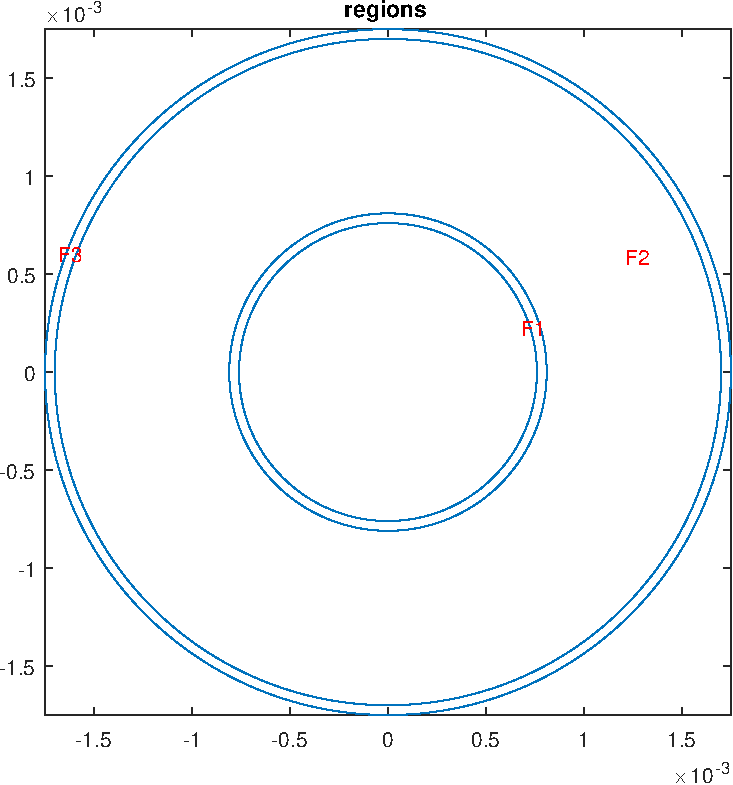
\includegraphics[width=\textwidth]{coaxial_regions.pdf}
      \caption{Περιοχές\vspace{1\baselineskip}}
      \label{fig:coaxial_regions}
  \end{subfigure}
  \hfill
  \begin{subfigure}[b]{0.3\textwidth}
      \centering
      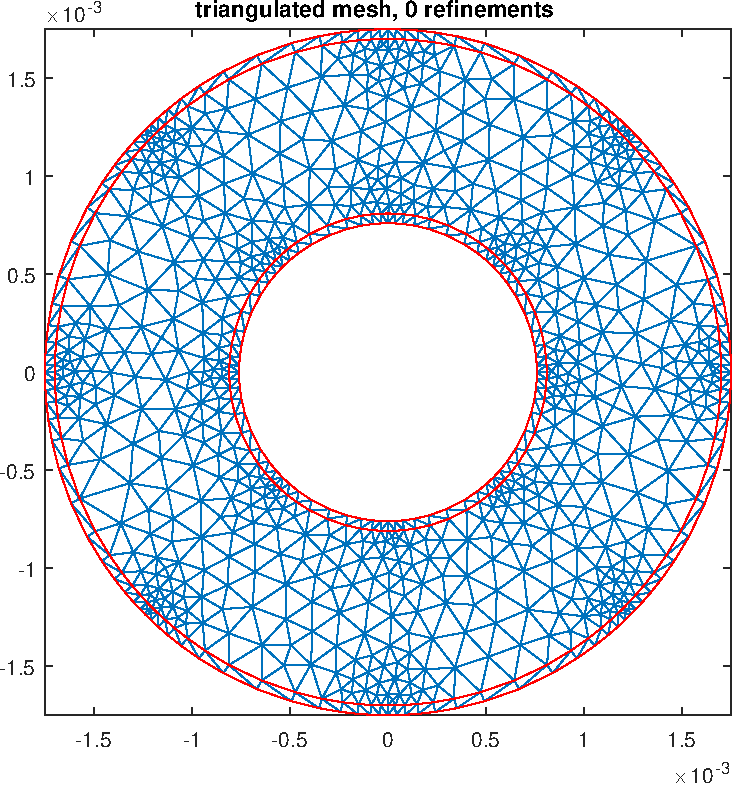
\includegraphics[width=\textwidth]{coaxial_mesh_0.pdf}
      \caption{Πλέγμα\vspace{1\baselineskip}}
      \label{fig:coaxial_mesh}
  \end{subfigure}
  \hfill
  \begin{subfigure}[b]{0.33\textwidth}
    \centering
    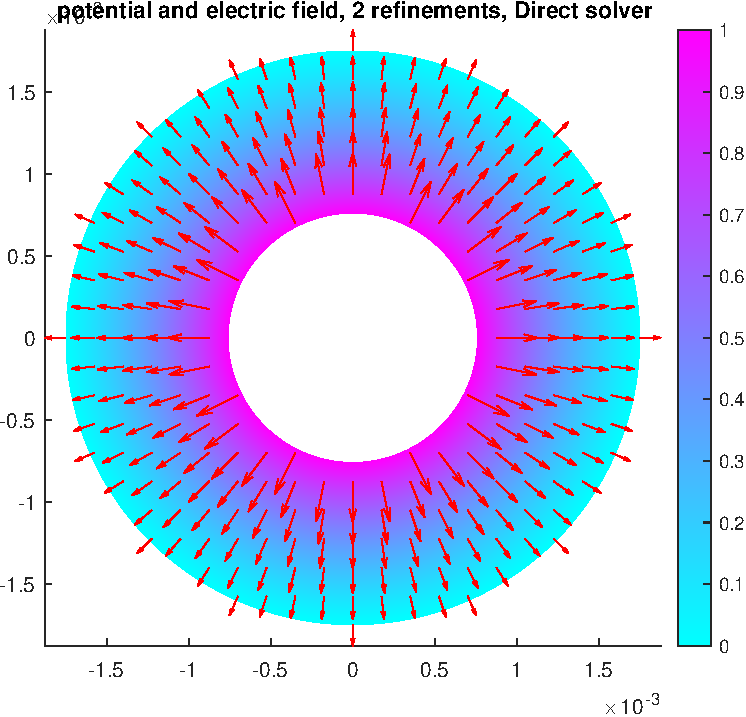
\includegraphics[width=\textwidth]{coaxial_field_2_Direct.pdf}
    \caption{Δυναμικό (χρώμα) και ηλεκτρικό πεδίο (βέλη).}
    \label{fig:coaxial_field}
\end{subfigure}
  \caption{}
  \label{}
\end{figure}



Το πρόβλημα λύνεται με 0,1,2 και 3 \en refinements \gr στο πλέγμα.
Το πλήθος βαθμών ελευθερίας σε κάθε περίπτωση είναι το πλήθος των άγνωστων κόμβων.
Για \en refinements \gr 0,1,2 και 3 είναι 761, 3228, 13280 και 53856 αντίστοιχα.
Στα γραφήματα δεν παρατηρείται διαφορά οπότε παρέχεται στο σχήμα \ref{fig:coaxial_field}
το αποτέλεσμα μόνο για 2 \en refinements. \gr 
Παρατηρείται ελάχιστη διαφορά στο αποτέλεσμα του υπολογισμού της χωρητικότητας, η 
οποία υπολογίζεται ως εξής:

Υπολογίζεται η ενέργεια ανά μονάδα μήκους με τη μέθοδο που παρουσιάστηκε παραπάνω. 
Έπειτα βρίσκεται η χωρητικότητα ανά μονάδα μήκους ως $C = 2 W_e / V^2$.

Το αποτέλεσμα για \en refinements \gr 0,1,2 και 3 είναι 
$66.8 \ pF/m$, $66.73 \ pF/m$, $66.706 \ pF/m$ 
και $66.7016 \ pF/m$, με σχετικό σφάλμα απο την αναλυτική τιμή [εξίσωση (\ref{eq:analytical_capacitance_coaxial})]
$0.15\%$, $0.0036\%$, $0.0076\%$ και $0.0003\%$
αντίστοιχα.
Με περισσότερα \en refinements \gr παίρνουμε ακριβέστερα αποτελέσματα.



Ο πίνακας $\mathbf{S}$ είναι αραιός (επειδή οι περισσότεροι κόμβοι είναι μη γειτονικοί
και για μη γειτονικούς κόμβους $\mathbf{S}[p,q]=0$). 
Επομένως μπορούμε να χρησιμοποιήσουμε \en iterative solver \gr ώστε να 
βελτιστοποιήσουμε μνήμη και χρόνο.
Χρησιμοποιήθηκε η συνάρτηση \en pcg \gr της \en matlab. \gr
Η \en iterative \gr μέθοδος παρουσιάζει πλεονέκτημα ως προς την ταχύτητα και τη μνήμη, όμως τα αποτελέσματα είναι λιγότερο ακριβή 
μιας ακολουθείται διαδικασία σύγκλισης. 

Χρησιμοποιήθηκε \en tolerance \gr στο σφάλμα ίσο με 0.01. Το αποτέλεσμα για 3 \en refinements \gr φαίνεται στο σχήμα \ref{fig:iterative_coaxial}
και όπως φαίνεται στα άκρα του καλωδίου παρουσιάζει οπτικό σφάλμα. Η υπολογισμένη χωρητικότητα ανά μονάδα μήκους με αυτή τη μέθοδο είναι 
$71.2 \ pF/m$ με μεγάλο σχετικό σφάλμα $6.87 \%$. 

Προφανώς εάν επιλεχθεί μικρότερο \en tolerance \gr σφάλματος το αποτέλεσμα 
θα είναι πολύ ακριβέστερο, επιλέχθηκε συγκεκριμένα αυτό για να επιδειχθούν 
τα πλεονέκτημα και μειονεκτήματα της μεθόδου: για 3 \en refinements \gr
η \en direct \gr μέθοδος τρέχει σε $0.072 sec$
ενώ η \en iterative \gr σε $0.048 sec$. Επίσης μπορεί να επιταχυνθεί περαιτέρω 
με καλό \en tuning \gr και παραλληλοποίηση. Για μεγαλύτερα σε πλήθος αγνώστων 
προβλήματα οι διαφορές θα ήταν εμφανέστερες. 

Για σύγκριση, στο 1 \en refinement, \gr σε μικρότερο χρόνο από την \en direct \gr
($0.00129sec$ έναντι $0.00292sec$) η \en iterative \gr υπολογίζει χωρητικότητα 
$66.887 \ pF/m$ με σχετικό σφάλμα $0.278 \%$, καλύτερη από ότι στα 3 \en refinements. \gr


\subsection*{Πυκνωτής παράλληλων πλακών}

Ο πυκνωτής απείρου μήκους του σχήματος \ref{fig:capacitor} με διαστάσεις $w = 4cm$, $t = 2mm$ και $d=1cm$, διηλεκτρικό με $\epsilon_r = 2.2$ 
τίθεται σε διαφορά δυναμικού $V = 100$ \en Volt. \gr Στις άκρες του υπολογιστικού χώρου υποτίθενται οριακές συνθήκες \en Neumann. \gr
Οι πλάκες έχουν οριακές συνθήκες \en Dirichlet \gr με τους κόμβους που ανήκουν στην άνω να έχουν δυναμικό $+V/2$ και αυτούς
που ανήκουν στην κάτω $-V/2$. Ορίζω υπολογιστικό χώρο διαστάσεων $5w \times 5w$.

Ο κώδικας \en matlab \gr βρίσκεται στο αρχείο \en capacitor.m. \gr
Ακολουθείται η ίδια διαδικασία με το ομοαξονικό καλώδιο (σχεδόν πανομοιότυπος κώδικας) για να υπολογιστούν το δυναμικό, το πεδίο και η χωρητικότητα. 
Διαφορά παρουσιάζεται στο γεγονός ότι η διηλεκτρική σταθερά εξαρτάται από την περιοχή (όπως φαίνεται στο σχήμα \ref{fig:capacitor} 
ανάμεσα στις πλάκες υπάρχει διηλεκτρικό με $\epsilon_r = 2.2 $ και έξω θεωρείται αέρας). Στο σχήμα
\ref{fig:capacitor_regions} φαίνονται οι περιοχές που ορίστηκαν. Η περιοχή \en F3 \gr ορίστηκε για να διαχωρίζεται η περιοχή με διαφορετικό διηλεκτρικό
και η \en F1 \gr για να διαχωρίζονται οι οριακοί κόμβοι (αυτοί που έχουν ένα ακμή στο όριο με την περιοχή 0)
σε αυτούς που έχουν 
συνθήκες \en Neumann \gr και και αυτούς με συνθήκες \en Dirichlet. \gr 
Η άνω πλάκα διαχωρίζεται από την κάτω από το γεγονός ότι οι κόμβοι της έχουν θετικές συντεταγμένες $y$, έναντι αρνητικών.

Στο σχήμα \ref{fig:capacitor_mesh} φαίνεται το πλέγμα και στο σχήμα \ref{fig:capacitor_potential} το δυναμικό μετά το πέρας της διαδικασίας.



\begin{figure}[h!]
  \centering
  \begin{subfigure}[b]{0.3\textwidth}
      \centering
      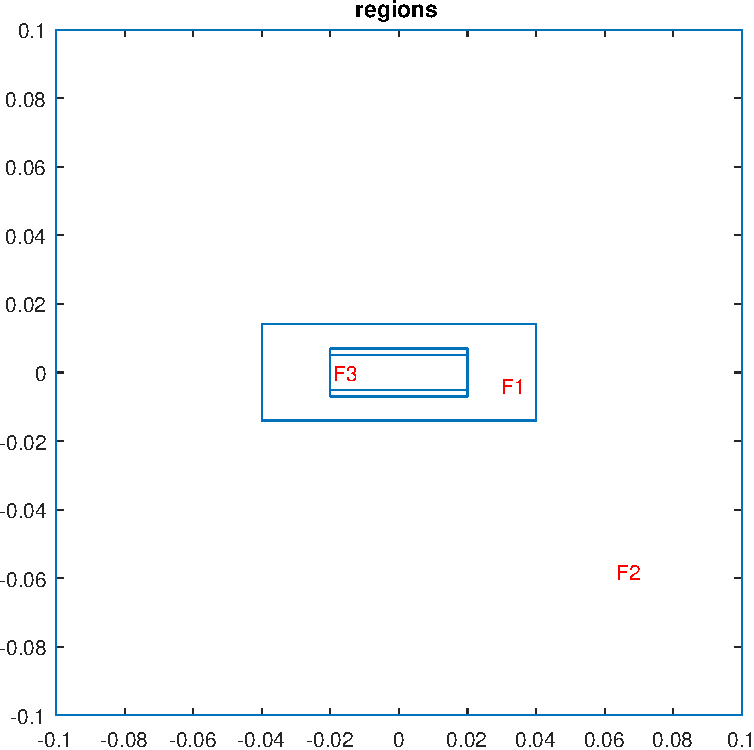
\includegraphics[width=\textwidth]{capacitor_regions_domain:5.pdf}
      \caption{Περιοχές}
      \label{fig:capacitor_regions}
  \end{subfigure}
  \hfill
  \begin{subfigure}[b]{0.3\textwidth}
      \centering
      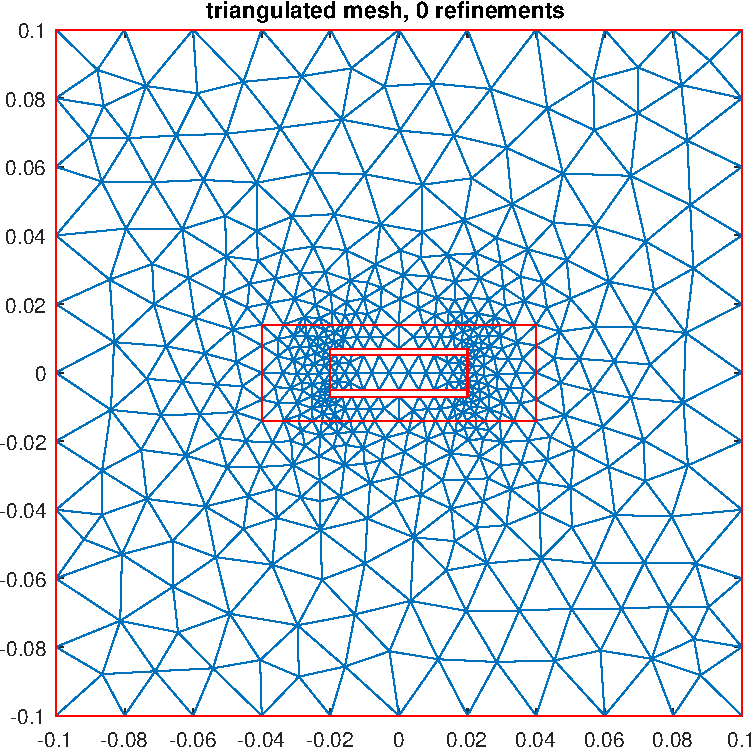
\includegraphics[width=\textwidth]{capacitor_mesh_0_domain:5.pdf}
      \caption{Πλέγμα}
      \label{fig:capacitor_mesh}
  \end{subfigure}
  \hfill
  \begin{subfigure}[b]{0.33\textwidth}
    \centering
    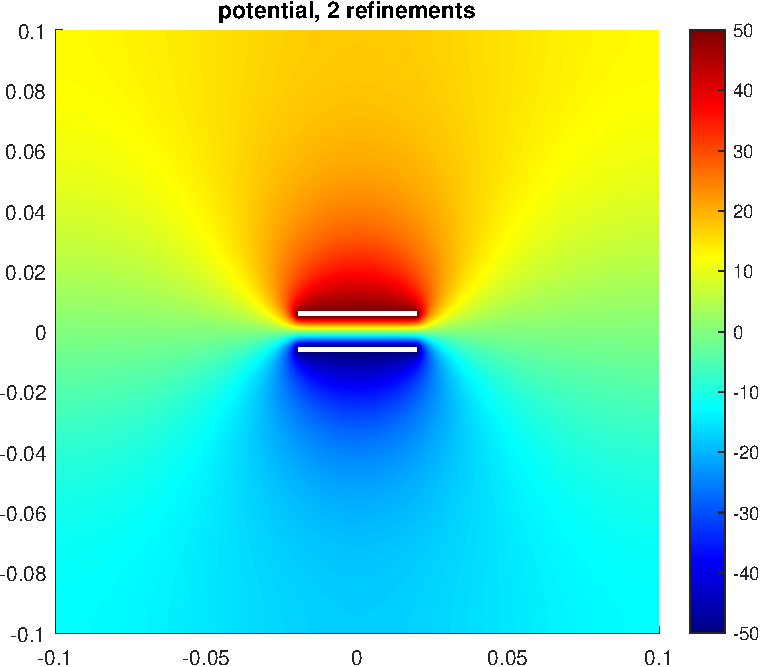
\includegraphics[width=\textwidth]{capacitor_potential_2_domain:5.pdf}
    \caption{Δυναμικό}
    \label{fig:capacitor_potential}
\end{subfigure}
  \caption{}
  \label{}
\end{figure}

Στο σχήμα \ref{fig:capacitor_field} φαίνεται το ηλεκτρικό πεδίο που υπολογίστηκε από τη σχέση $\mathbf{E} = - \nabla \phi$. 

\begin{figure}[h!]
  \centering
  \begin{subfigure}[b]{0.44\textwidth}
      \centering
      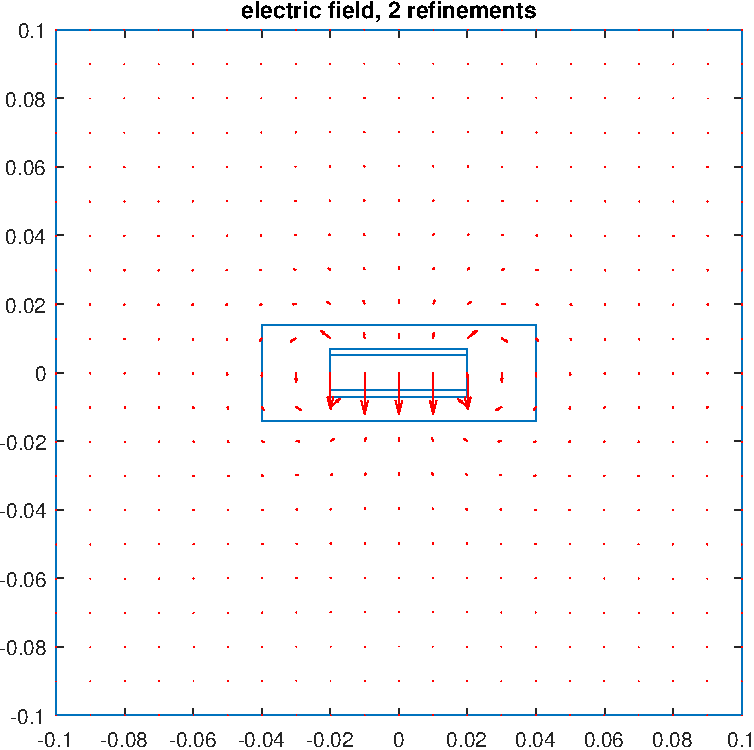
\includegraphics[width=\textwidth]{capacitor_field_2_domain:5.pdf}
      \caption{Ηλεκτρικό πεδίο πυκνωτή παράλληλων πλακών \vspace{\baselineskip}}
      \label{}
  \end{subfigure}
  \hfill
  \begin{subfigure}[b]{0.5\textwidth}
    \centering
    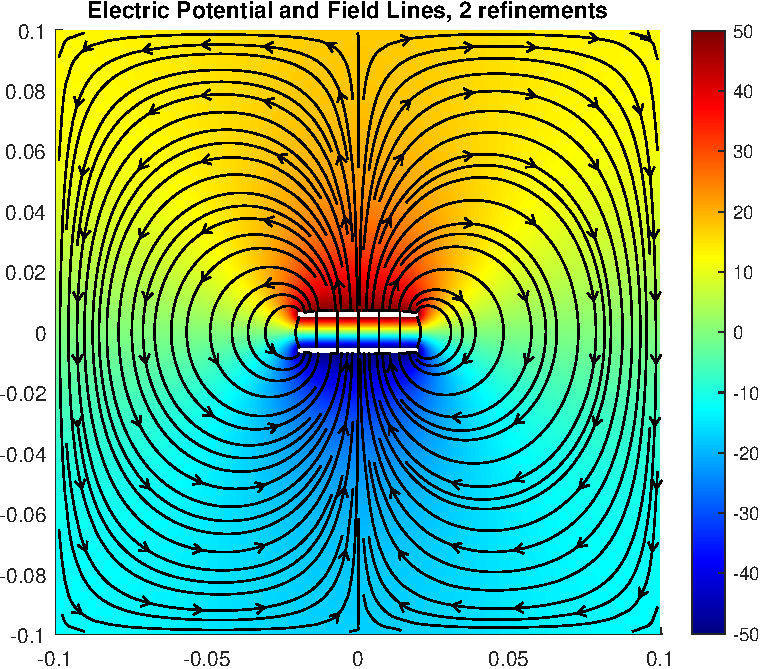
\includegraphics[width=\textwidth]{capacitor_field_streamlines_2_domain:5.pdf}
    \caption{Δυναμικό (χρώμα) και ηλεκτρικό πεδίο (γραμμές ροής) πυκνωτή παράλληλων πλακών}
    \label{}
\end{subfigure}
  \caption{}
  \label{fig:capacitor_field}
\end{figure}


\subsubsection*{Χωρητικότητα}

Θεωρώντας ότι το πλάτος $w$ είναι πολύ μεγαλύτερο από την απόσταση $d$ 
μπορούμε να καταλήξουμε σε μία αναλυτική σχέση για τον υπολογισμό της 
χωρητικότητας:

\begin{equation}    \label{eq:parallel_plate_analytical_capacitance}
  C = \epsilon \frac{A}{d}
\end{equation}
όπου $A$ το εμβαδόν της πλάκας και $d$ η απόσταση μεταξύ των πλακών.  
Επομένως η ανά μονάδα χωρητικότητα στο παραπάνω πρόβλημα θα είναι: 
\begin{equation}
  C = \epsilon \frac{w}{d} = 77.9 \ pF/m
\end{equation}

Αυτή η σχέση υποθέτει ότι δεν υπάρχουν φαινόμενα άκρων και ότι το πεδίο είναι 
συγκεντρωμένο στο εσωτερικό του πυκνωτή. Όπως φαίνεται στα σχήματα 
\ref{fig:capacitor} και \ref{fig:capacitor_field} οι υποθέσεις αυτές δεν ισχύουν.

Υπολογίζοντας την χωρητικότητα ανά μονάδα μήκους μην υιοθετώντας αυτές τις υποθέσεις με 
τη χρήση \en FEM \gr όπως και προηγουμένως,
τα αποτελέσματα
για 0,1,2 και 3 \en refinements \gr είναι 
$92.88 \ pF/m$, $92.37 \ pF/m$, $92.20 pF/m$ και $92.14 \ pF/m$
αντίστοιχα. Φαίνεται με την αύξηση των \en refinements \gr να συγκλίνει ομοιόμορφα σε μια τιμή.



Έπειτα εξετάζουμε την επιρροή του μεγέθους του υπολογιστικού χώρου. Χρησιμοποιώντας 2 \en refinements \gr λύνουμε το πρόβλημα 
για υπολογιστικό χώρο διαστάσεων $3w \times 3w$, $5w \times 5w$, $7w \times 7w$ και $9w \times 9w$.
Οι τιμές χωρητικότητας ανά μονάδα μήκους προκύπτουν:
$91.40 \ pF/m$, $92.20 \ pF/m$, $92.42 \ pF/m$ και $92.51 \ pF/m$
αντίστοιχα.
Με την αύξηση των διαστάσεων του υπολογιστικού χώρου φαίνεται επίσης να συγκλίνει 
ομοιόμορφα σε μία τιμή. 

Το γεγονός αυτό της σύγκλισης της χωρητικότητας ανά μονάδα μήκους με την αύξηση των διαστάσεων του υπολογιστικού χώρου ερμηνεύεται ως εξής:
Σε αντίθεση με το ομοαξονικό καλώδιο, η επιρροή του πυκνωτή παράλληλων πλακών εκτίνεται στο άπειρο (η ένταση του ηλεκτρικού πεδίου 
μειώνεται τετραγωνικά όμως δεν μηδενίζεται πουθενά) επομένως για να υπολογίσουμε την ενέργεια ανά μονάδα μήκους σύμφωνα με την 
(\ref{eq:We}) πρέπει να ολοκληρώσουμε στο άπειρο. Δεν έχουμε αυτή την δυνατότητα, όμως εφόσον το πεδίο εξασθενεί τετραγωνικά,
με την αύξηση των διαστάσεων του χώρου ολοκλήρωσης (υπολογιστικός χώρος) το ολοκλήρωμα θα συγκλίνει ομοιόμορφα. Έτσι μπορούμε να επιτύχουμε 
αρκετά ακριβή αποτελέσματα μεγαλώνοντας τον υπολογιστικό χώρο. 

(Η ομοιομορφία εξασφαλίζεται από το γεγονός ότι αυξάνοντας τον χώρο ολοκλήρωσης, επειδή η προς ολοκλήρωση ποσότητα
$\epsilon |\mathbf{E}|^2$ είναι παντού θετική, το ολοκλήρωμα θα αυξάνεται συνεχώς, όμως με φθίνων ρυθμό,
πλησιάζοντας την πραγματική ποσότητα.
Έτσι δεν είναι δυνατόν με αύξηση του χώρου ολοκλήρωσης να αυξηθεί το σφάλμα).

Βλέπουμε τώρα ότι υπάρχει μεγάλη απόκλιση των αποτελεσμάτων \en FEM \gr και 
σχέσης (\ref{eq:parallel_plate_analytical_capacitance}), η οποία οφείλεται 
στα φαινόμενα άκρων τα οποία η (\ref{eq:parallel_plate_analytical_capacitance})
αγνοεί. 

Συμπεραίνουμε λοιπόν ότι για το συγκεκριμένο πρόβλημα ήταν απαραίτητη η χρήση 
υπολογιστικής μεθόδου.

\pagebreak
\subsubsection*{Επιπλέον γραφήματα}

% extra figures------------- more refines......, iterative coaxial
\begin{figure}[h!]
  \centering
  \begin{subfigure}[b]{0.3\textwidth}
      \centering
      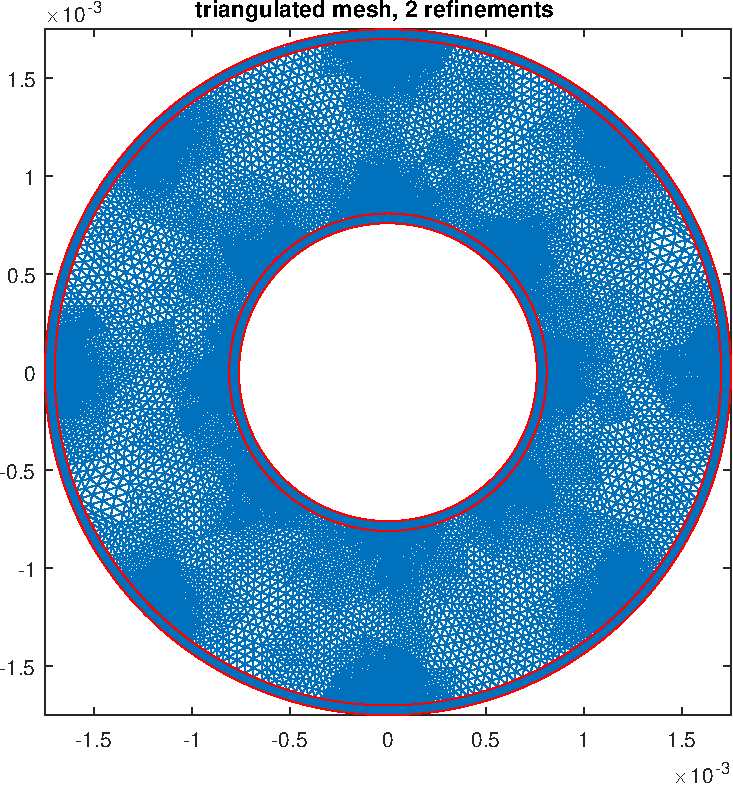
\includegraphics[width=\textwidth]{coaxial_mesh_2.pdf}
      \caption{Πλέγμα ομοαξονικού καλωδίου με 2 \en refinements. \gr \vspace{1\baselineskip}}
      \label{fig:coaxial_2_refinements}
  \end{subfigure}
  \hfill
  \begin{subfigure}[b]{0.3\textwidth}
      \centering
      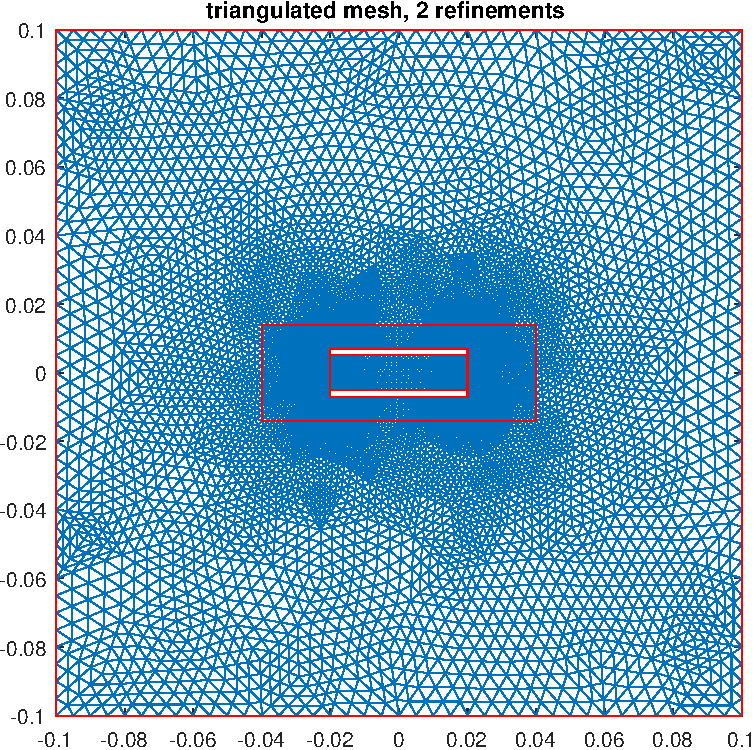
\includegraphics[width=\textwidth]{capacitor_mesh_2_domain:5.pdf}
      \caption{Πλέγμα πυκνωτή παράλληλων πλακών με 2 \en refinements. \gr \vspace{2\baselineskip}}
      \label{fig:capacitor_2_refinements}
  \end{subfigure}
  \hfill
  \begin{subfigure}[b]{0.33\textwidth}
    \centering
    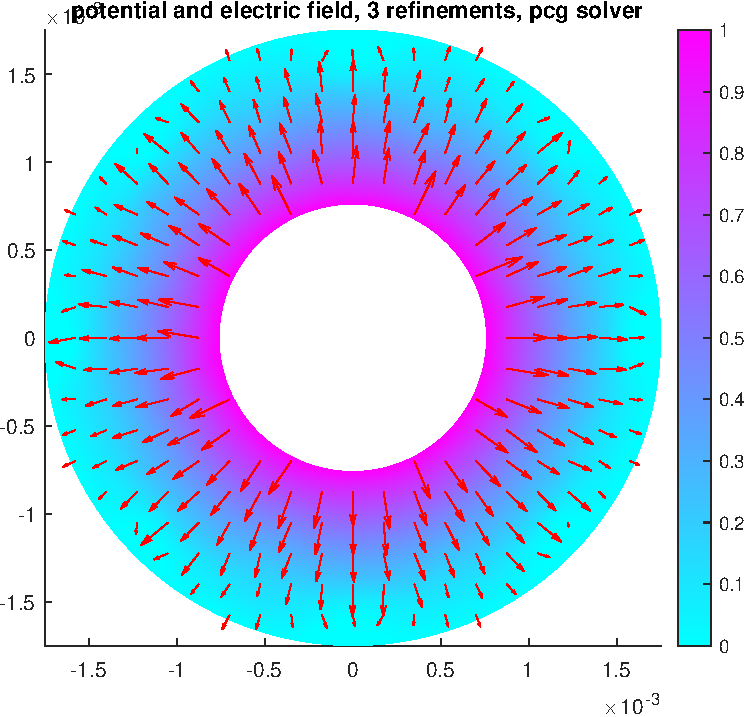
\includegraphics[width=\textwidth]{coaxial_field_3_pcg.pdf}
    \caption{Δυναμικό (χρώμα) και ηλεκτρικό πεδίο (βέλη) του ομοαξονικού καλωδίου με \en iterative solver.\gr }
    \label{fig:iterative_coaxial}
\end{subfigure}
  \caption{Επιπλέον γραφήματα}
  \label{fig:extra_1}
\end{figure}










\section*{Μέρος Β}


\subsection*{Κυματοδηγός κυκλικής διατομής}


Βρίσκουμε τους εννέα πρώτους ρυθμούς (είτε ΤΕ είτε ΤΜ) ενός κυλινδρικού κυματοδηγού
ακτίνας $a = 1 \ cm$. 
Οι ρυθμοί υπολογίζονται ξεχωριστά για ΤΕ και ΤΜ και επιστρέφονται οι 9 μικρότεροι. 

Ο αλγόριθμος \en FEM \gr είναι ο εξής:
Λύνεται το πρόβλημα ιδιοτιμών:

\begin{equation}   \label{eq:eigen_system}
  \begin{split}
    TE: \ \ \ (\mathbf{S} - k_c^2\mathbf{T})\mathbf{H} = \mathbf{0} \\
    TM: \ \ \ (\mathbf{S} - k_c^2\mathbf{T})\mathbf{Ε} = \mathbf{0}
  \end{split}
\end{equation}

Με τον πίνακα $\mathbf{S}$ να υπολογίζεται όπως προηγουμένως, όμως χωρίς τη διηλεκτρική σταθερά, δηλαδή:

\[\mathbf{S}[p,q] =  \sum_{t | p,q \in t}  (b_ib_j + c_ic_j) A_e  \]

και $\mathbf{T}$ είναι ο πίνακας μάζας που δίνεται από την
\[\mathbf{T}[p,q] =  \sum_{t | p,q \in t}
\begin{cases}
    A_e / 6, & p=q \\
    A_e / 12, & p \neq q
\end{cases}
 \]


Η λύση σε κάθε περίπτωση θα είναι ο πίνακας $\mathbf{H}$ ή $\mathbf{E}$ και η ιδιοτιμή $k_c^2$ που του αντιστοιχεί. Οι πίνακες $\mathbf{H}$, $\mathbf{E}$
(πίνακες στήλη) περιέχουν για κάθε κόμβο του πλέγματος την τιμή των $H_z, E_z$, δηλαδή τα πλάτος των αντίστοιχων πεδίων κατά τη διεύθυνση διάδοσης.

\subsubsection*{Οριακές συνθήκες}

Στην περίπτωση των ΤΕ ρυθμών, λύνουμε ώς προς $\mathbf{H}$, το οποίο έχει ομογενής \en Neumann \gr οριακές συνθήκες στο όριο. Επομένως όλοι οι κόμβοι 
αφήνονται ελεύθεροι και το σύστημα δε χρειάζεται επεξεργασία.

Στην περίπτωση των ΤΜ ρυθμών, λύνουμε ως προς $\mathbf{E}$, το οποίο στο όριο έχει ομογενής συνθήκες \en Dirchlet. \gr 
Έτσι πρέπει, όπως και στο ηλεκτροστατικό πρόβλημα, να αναλυθούν τα $\mathbf{E}$, $\mathbf{S}$ και $\mathbf{T}$ στους γνωστούς και άγνωστους κόμβους:
\[\mathbf{E} = 
  \left[ \begin{array}{@{}c@{}}
  \mathbf{E}_f \\
  \hline
  \mathbf{E}_p
  \end{array} \right], \ \ \ \ \ \mathbf{S} = 
  \left[ \begin{array}{@{}c|c@{}}
    \mathbf{S}_{ff} & \mathbf{S}_{fp} \\
    \hline
    \mathbf{S}_{pf} & \mathbf{S}_{pp}
    \end{array} \right], \ \ \ \ \ \mathbf{T} = 
    \left[ \begin{array}{@{}c|c@{}}
      \mathbf{T}_{ff} & \mathbf{T}_{fp} \\
      \hline
      \mathbf{T}_{pf} & \mathbf{T}_{pp}
      \end{array} \right]
  \]

Τότε το σύστημα γίνεται:

\[ \left(
  \left[ \begin{array}{@{}c|c@{}}
    \mathbf{S}_{ff} & \mathbf{S}_{fp} \\
    \hline
    \mathbf{S}_{pf} & \mathbf{S}_{pp}
    \end{array} \right] - k_c^2 
    \left[ \begin{array}{@{}c|c@{}}
      \mathbf{T}_{ff} & \mathbf{T}_{fp} \\
      \hline
      \mathbf{T}_{pf} & \mathbf{T}_{pp}
      \end{array} \right]
  \right)
  \cdot \left[ \begin{array}{@{}c@{}}
    \mathbf{E}_f \\
    \hline
    \mathbf{E}_p
    \end{array} \right] = \mathbf{0}    \Rightarrow
\]

\[
  \left[ \begin{array}{@{}c|c@{}}
    \mathbf{S}_{ff} - k_c^2 \mathbf{T}_{ff} & \mathbf{S}_{fp} - k_c^2 \mathbf{T}_{fp} \\
    \hline
    \mathbf{S}_{pf} - k_c^2 \mathbf{T}_{pf} & \mathbf{S}_{pp} - k_c^2 \mathbf{T}_{pp}
    \end{array} \right]
\cdot \left[ \begin{array}{@{}c@{}}
  \mathbf{E}_f \\
  \hline
  \mathbf{E}_p
  \end{array} \right] = \mathbf{0}  \Rightarrow
\]

\[
  \left[ \begin{array}{@{}c@{}}
    (\mathbf{S}_{ff} - k_c^2 \mathbf{T}_{ff}) \cdot \mathbf{E}_f + (\mathbf{S}_{fp} - k_c^2 \mathbf{T}_{fp}) \cdot \mathbf{E}_p\\
    \hline
    (\mathbf{S}_{pf} - k_c^2 \mathbf{T}_{pf}) \cdot \mathbf{E}_f + (\mathbf{S}_{pp} - k_c^2 \mathbf{T}_{pp}) \cdot \mathbf{E}_p
    \end{array} \right] = \mathbf{0}  
\]
 
Από τη συμμετρία, αρκεί να λύσουμε το πάνω μέρος:

\[(\mathbf{S}_{ff} - k_c^2 \mathbf{T}_{ff}) \cdot \mathbf{E}_f + (\mathbf{S}_{fp} - k_c^2 \mathbf{T}_{fp}) \cdot \mathbf{E}_p = \mathbf{0}\]


και επειδή στο όριο το ηλεκτρικό πεδίο είναι 0, δηλαδή $\mathbf{E}_p = 0$, προκύπτει:

\begin{equation} \label{eq:eigen_system}
  (\mathbf{S}_{ff} - k_c^2 \mathbf{T}_{ff}) \cdot \mathbf{E}_f = \mathbf{0}
\end{equation}


\subsubsection*{Υπόλοιπες συνιστώσες}

Έχοντας βρει το $H_z$ για ΤΕ και $E_z$ για ΤΜ μπορούμε να υπολογίσουμε τις υπόλοιπες συνιστώσες:\footnote{Οι τύποι έχουν παρθεί από
το βιβλίο ΜΙΚΡΟΚΥΜΑΤΑ θεωρία και εφαρμογές των Τραϊανός Β. Γιούλτσης, Εμμανουήλ Ε. Κριεζής, σελ. 136, με επεξεργασία για ΤΕ και ΤΜ ρυθμούς}


\begin{equation} \label{eq:rest_coords}
  \begin{aligned}
    \text{TE}: \ \ \ \ \ & &     \ \ \ \ \ \ \  \text{TM}: \ \ \ \ \ & & \\ 
    E_x &= - &\frac{j \omega \mu}{k_c^2} \frac{\partial H_z}{\partial y} \ \ \ \ \ \ \ \ \ \ \ \ \ \ \ \ \ \         E_x &= - &\frac{j \beta}{k_c^2} \frac{\partial E_z}{\partial x}  \\ 
    E_y &=  &\frac{j \omega \mu}{k_c^2} \frac{\partial H_z}{\partial x} \ \ \ \ \ \ \ \ \ \ \ \ \ \ \ \  \  \        E_y &= - &\frac{j \beta}{k_c^2} \frac{\partial E_z}{\partial y}  \\ 
    H_x &= - &\frac{j \beta}{k_c^2} \frac{\partial H_z}{\partial x}  \ \ \ \ \ \ \ \ \ \ \ \ \ \ \ \ \ \         H_x &=   &\frac{j \omega \epsilon }{k_c^2} \frac{\partial E_z}{\partial y} \\ 
    H_y &= - &\frac{j \beta}{k_c^2} \frac{\partial H_z}{\partial y}   \ \ \ \ \ \ \ \ \ \ \ \ \ \ \ \ \ \ \     H_y &= - &\frac{j \omega \epsilon }{k_c^2} \frac{\partial E_z}{\partial x}  \\ 
  \end{aligned}
\end{equation}




\subsubsection*{Υλοποίηση}

Αφού υλοποιηθεί η μέθοδος πεπερασμένων στοιχείων στο \en MATLAB \gr παίρνουμε τους πρώτους 12 ΤΕ ρυθμούς (μικρότερης ιδιοτιμή)
οι οποίοι φαίνονται στο σχήμα \ref{fig:TE_12_first}. 


\begin{figure}[h]
  \centering
  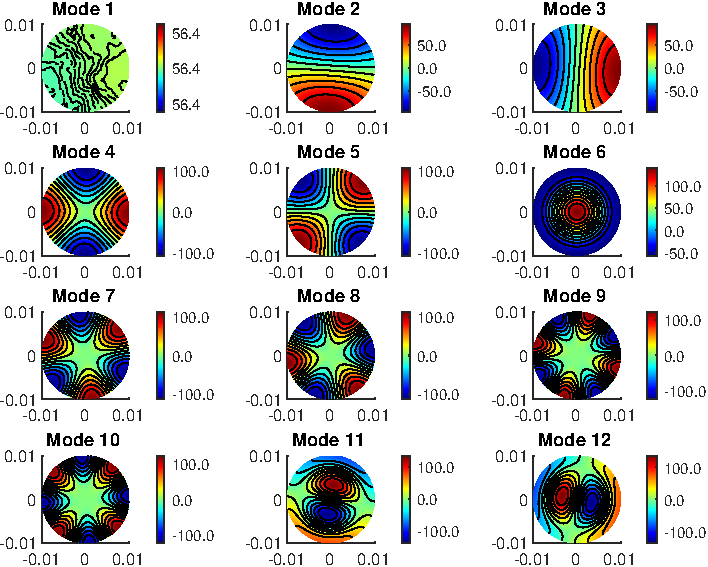
\includegraphics[width=0.7\textwidth]{TE_first_12_modes.pdf}
  \caption{Το αποτέλεσμα της μεθόδου για πρώτους 12 ρυθμούς ΤΕ}
  \label{fig:TE_12_first}
\end{figure}


Για κάθε ρυθμό (ιδιοδιάνυσμα) το πρόγραμμα μας δίνει και την ιδιοτιμή του 
$k_c^2$ (βλ. εξίσωση (\ref{eq:eigen_system}) ).
Μπορούμε να υπολογίσουμε την συχνότητα αποκοπής των ρυθμών ως
\[f_c = \frac{c}{2 \pi}k_c\]
Οι τιμές της συχνότητας αποκοπής για τους πρώτους 12 ρυθμούς ΤΕ που βρήκαμε είναι: \\
$[0, 0.8788, 0.8788, 1.4583,1.4583, 1.8304, 2.0067,2.0068,2.5415, 2.5416,2.5489,2.5491
] \cdot 10^{10} \ Hz$

Η πρώτη συχνότητα των 0 \textlatin{Hz}, με $H_z$ σταθερό όπως φαίνεται στο σχήμα \ref{fig:TE_12_first}
παραπέμπει σε ΤΕΜ ρυθμό και απορρίπτεται. Έπειτα βλέπουμε ότι πολλοί ρυθμοί εμφανίζονται 
σε δυάδες με ίδια περίπου συχνότητα, και $H_z$ ίδιο με κάποια στροφή. 
Αυτοί αποτελούν εκφυλισμένους ρυθμούς και απορρίπτουμε τον έναν απο τους δύο.

Αφού κάνουμε την ίδια διαδικασία για ρυθμούς ΤΜ και κρατήσουμε τους συνολικά 
9 πρώτους (μικρότερη συχνότητα αποκοπής) λαμβάνουμε τους:

\begin{figure}[h]
  \centering
  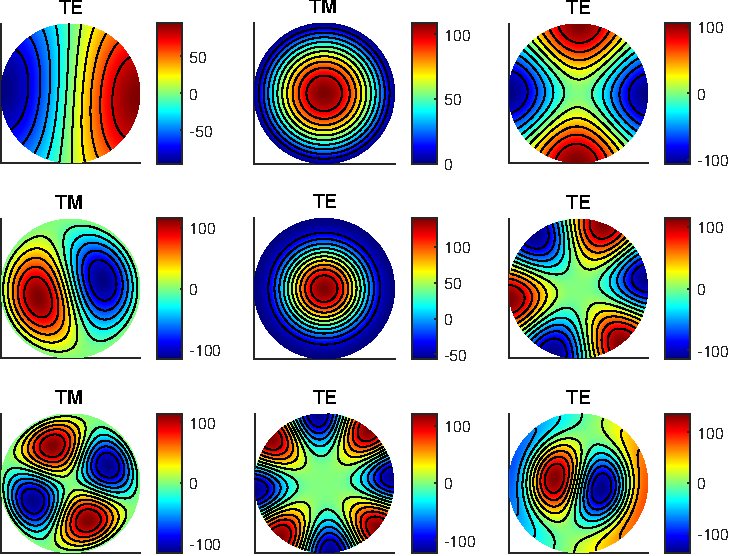
\includegraphics[width=0.7\textwidth]{Waveguide_first_nine_modes.pdf}
  \caption{Οι 9 πρώτοι ρυθμοί. Απεικονίζεται το πλάτος του πεδίου που βρίσκεται στην 
  διεύθυνση μετάδοσης, $E_z$ για ΤΜ και $H_z$ για ΤΕ.}
  \label{fig:9modes}
\end{figure}


Υπολογίζω και τις εγκάρσιες συνιστώσες με τις 
εξισώσεις (\ref{eq:rest_coords}). Συγκεκριμένα εφόσον εξαρτώνται από τη 
συχνότητα όμως εμείς δεν λύνουμε για κάποια  συγκεκριμένη συχνότητα, 
υπολογίζω χωρίς τις σταθερές, δηλαδή παίρνοντας υπόψη μόνο τις παραγώγους και 
τα πρόσημα. Έτσι το αποτέλεσμα είναι κάποια ποσότητα $\alpha\mathbf{E}_t$ που συμβολίζει 
κάτι ανάλογο στο $\mathbf{E}_t$, εφόσον θα τις απεικονίσουμε με διαγράμματα ροής 
το πλάτος δεν επηρεάζει.

Στο σχήμα \ref{fig:9modes_trans} φαίνονται οι δυναμικές γραμμές τους.



\begin{figure}[h]
  \centering
  \includegraphics[width=0.65\textwidth]{Waveguide_first_nine_modes_transverse.pdf}
  \caption{Οι 9 πρώτοι ρυθμοί. Απεικονίζονται οι δυναμικές γραμμές των 
  εγκάρσιων συνιστωσών, με μπλε το ηλεκτρικό πεδίο και με μαύρο το μαγνητικό.}
  \label{fig:9modes_trans}
\end{figure}



Οι συχνότητες αποκοπής υπολογίζονται αναλυτικά ως 
\[f_c^{TE_{nm}} = \frac{c}{2 \pi a} p_{nm}' \ \ \ \ f_c^{TM_{nm}} = \frac{c}{2 \pi a} p_{nm}\]
με $a$ την ακτίνα, $p_{nm}'$  τις ρίζες των συναρτήσεων \en Bessel \gr με πρώτες τιμές:
\[
\begin{matrix}
  \hline 
  \mathbf{m} \backslash \mathbf{n} & \mathbf{0} & \mathbf{1} & \mathbf{2} & \mathbf{3} & \mathbf{4}\\ 
  \hline 
  \mathbf{1} & 3.832 & 1.841 & 3.054 & 4.201 & 5.3175 \\
  \mathbf{2} & 7.016 & 5.331 & 6.706 & 8.015 & 9.2824\\
  \mathbf{3} & 10.173 & 8.536 & 9.969 & 11.346 & 12.6819\\
  \hline
\end{matrix}
\]
και $p_{nm}$ τα μηδενικά των συναρτήσεων \en Bessel, \gr με πρώτες τιμές:
\[
\begin{matrix}
  \hline 
  \mathbf{m} \backslash \mathbf{n} & \mathbf{0} & \mathbf{1} & \mathbf{2} & \mathbf{3} \\
  \hline 
  \mathbf{1} & 2.405 & 3.832 & 5.135 & 6.380 \\
  \mathbf{2} & 5.520 & 7.016 & 8.417 & 9.761 \\
  \mathbf{3} & 8.654 & 10.174 & 11.620 & 13.020 \\
  \hline
\end{matrix}
\]

Προκύπτουν αναλυτικά οι 9 μικρότερες συχνότητες αποκοπής:
\[
\begin{matrix}
  \hline
  TE_{11}: &  0.8784 &\cdot 10^{10} \ Hz \\
  TM_{01}: & 1.147 &\cdot 10^{10} \ Hz \\
  TE_{21}: & 1.457 &\cdot 10^{10} \ Hz \\
  TM_{11}: & 1.829 &\cdot 10^{10} \ Hz \\
  TE_{01}: & 1.828 &\cdot 10^{10} \ Hz \\
  TE_{31}: & 2 &\cdot 10^{10} \ Hz \\
  TM_{21}: & 2.45 &\cdot 10^{10} \ Hz \\
  TE_{41}: & 2.537 &\cdot 10^{10} \ Hz \\
  TE_{12}: & 2.544 &\cdot 10^{10} \ Hz \\
  \hline
\end{matrix}
\]

Οι 9 μικρότερες συχνότητες αποκοπής που μας επιστρέφει το πρόγραμμα είναι οι:
\[ [0.8788, 1.1479, 1.4583, 1.8300, 1.8304, 2.0067, 2.4546, 2.5415, 2.5489] \ \cdot 10^{10} \ Hz \]



Συγκρίνοντας και το σχήμα \ref{fig:9modes_trans}
με το σχήμα 
\ref{fig:given} που μας δίνεται, βλέπουμε ότι έχουμε 
αναγνωρίσει σωστά τους πρώτους 9 ρυθμούς.

\begin{figure}[h]
  \centering
  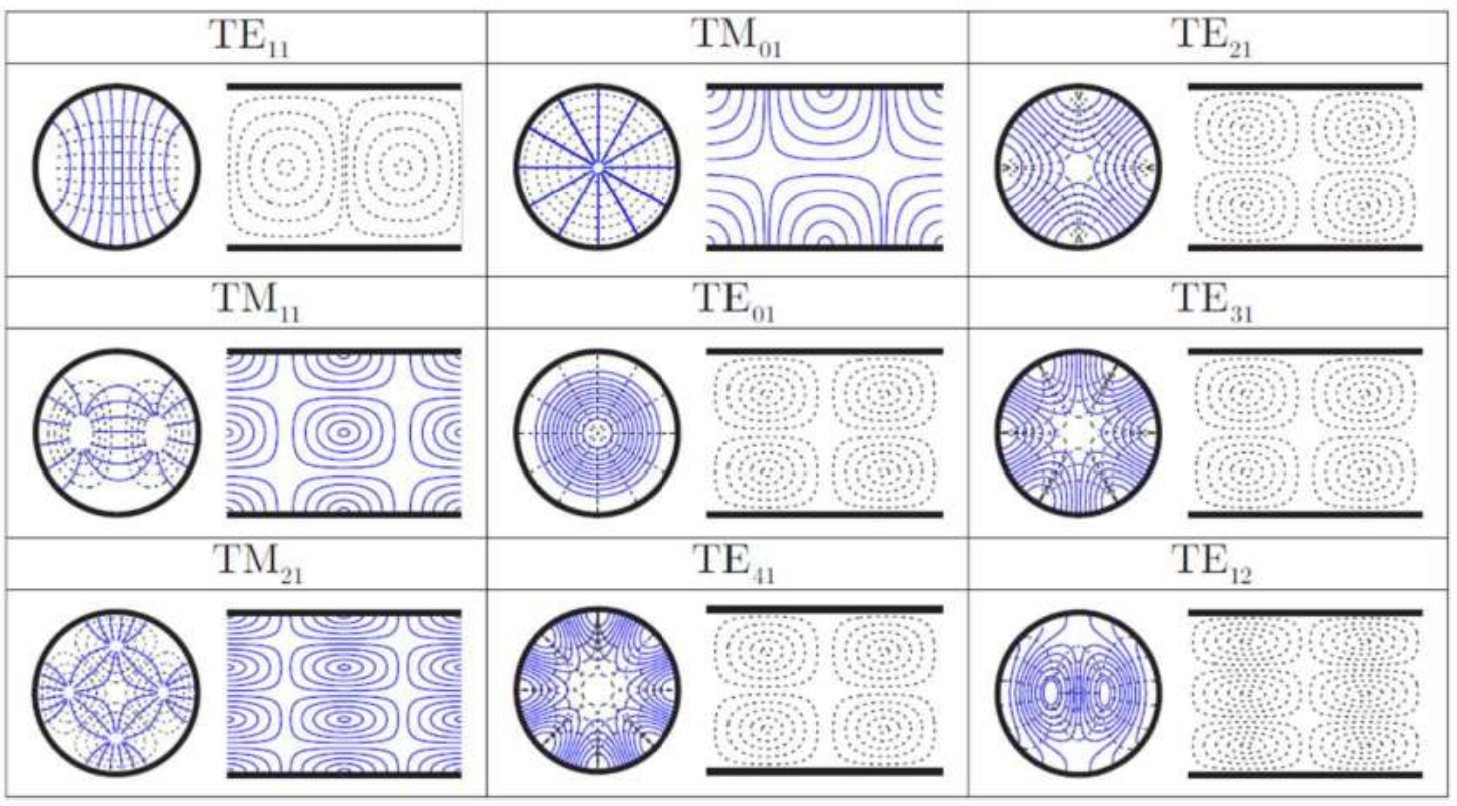
\includegraphics[width=0.65\textwidth]{given.png}
  \caption{}
  \label{fig:given}
\end{figure}

Συγκρίνοντας τα διαγράμματα \ref{fig:9modes} και \ref{fig:9modes_trans} βλέπουμε ότι οι ισοσταθμικές των πεδίων στην διεύθυνση μετάδοσης (\ref{fig:9modes})
συμπίπτουν με τις δυναμικές γραμμές (\ref{fig:9modes_trans}) του εγκάρσιου πεδίου, (του Ε στα ΤΕ και του Μ στα ΤΜ). 
Αυτό το καταλαβαίνουμε διότι οι ισοσταθμικές μιας συνάρτησης είναι παντού κάθετες στην κλήση της, και από τις εξισώσεις 
(\ref{eq:rest_coords}) βλέπουμε ότι στα ΤΕ το εγκάρσιο $\mathbf{E}_t$ είναι κάθετο στην κλίση του $H_z$ και στα ΤΜ το εγκάρσιο $\mathbf{H}_t$ είναι 
κάθετο στην κλίση του $E_z$ ($H_x$ ανάλογο της κλίσης του $E_z$ ως προς $y$ και $H_y$ ανάλογο της κλίσης ως προς $x$.)


Στον παρακάτω πίνακα αναγράφονται οι υπολογισμένες συχνότητες αποκοπής για \en refinements \gr 0,1,2 και 3, η αναλυτική τιμή των 
συχνοτήτων αποκοπής και το σχετικό σφάλμα. 

\en 
\begin{center}
  

  \begin{tabular}{|c|c|c|c|c|}
    \hline
    \textbf{Refinement amount} & \textbf{Mode} & \textbf{Analytical (Hz)} & \textbf{Numerical (Hz)} & \textbf{Error (\%)} \\
    \hline
    \multirow{9}{*}{0} 
    & $TE_{11}$ & $0.8784 \times 10^{10}$ Hz & $0.8833 \times 10^{10}$ Hz & 0.56 \\
    & $TM_{01}$ & $1.147 \times 10^{10}$ Hz  & $1.1546 \times 10^{10}$ Hz & 0.66 \\
    & $TE_{21}$ & $1.457 \times 10^{10}$ Hz  & $1.4726 \times 10^{10}$ Hz & 1.07 \\
    & $TM_{11}$ & $1.828 \times 10^{10}$ Hz  & $1.8546 \times 10^{10}$ Hz & 1.46 \\
    & $TE_{01}$ & $1.828 \times 10^{10}$ Hz  & $1.8621 \times 10^{10}$ Hz & 1.88 \\
    & $TE_{31}$ & $2.000 \times 10^{10}$ Hz  & $2.0386 \times 10^{10}$ Hz & 1.93 \\
    & $TM_{21}$ & $2.450 \times 10^{10}$ Hz  & $2.5169 \times 10^{10}$ Hz & 2.73 \\
    & $TE_{41}$ & $2.537 \times 10^{10}$ Hz  & $2.6049 \times 10^{10}$ Hz & 2.68 \\
    & $TE_{12}$ & $2.544 \times 10^{10}$ Hz  & $2.6234 \times 10^{10}$ Hz & 3.12 \\
    \hline
    
    \multirow{9}{*}{1} 
    & $TE_{11}$ & $0.8784 \times 10^{10}$ Hz & $0.8797 \times 10^{10}$ Hz & 0.15 \\
    & $TM_{01}$ & $1.147 \times 10^{10}$ Hz  & $1.1492 \times 10^{10}$ Hz & 0.19 \\
    & $TE_{21}$ & $1.457 \times 10^{10}$ Hz  & $1.4612 \times 10^{10}$ Hz & 0.29 \\
    & $TM_{11}$ & $1.828 \times 10^{10}$ Hz  & $1.8350 \times 10^{10}$ Hz & 0.33 \\
    & $TE_{01}$ & $1.828 \times 10^{10}$ Hz  & $1.8368 \times 10^{10}$ Hz & 0.48 \\
    & $TE_{31}$ & $2.000 \times 10^{10}$ Hz  & $2.0132 \times 10^{10}$ Hz & 0.66 \\
    & $TM_{21}$ & $2.450 \times 10^{10}$ Hz  & $2.4673 \times 10^{10}$ Hz & 0.71 \\
    & $TE_{41}$ & $2.537 \times 10^{10}$ Hz  & $2.5545 \times 10^{10}$ Hz & 0.69 \\
    & $TE_{12}$ & $2.544 \times 10^{10}$ Hz  & $2.5640 \times 10^{10}$ Hz & 0.79 \\
    \hline
    
    \multirow{9}{*}{2} 
    & $TE_{11}$ & $0.8784 \times 10^{10}$ Hz & $0.8788 \times 10^{10}$ Hz & 0.05 \\
    & $TM_{01}$ & $1.147 \times 10^{10}$ Hz  & $1.1479 \times 10^{10}$ Hz & 0.08 \\
    & $TE_{21}$ & $1.457 \times 10^{10}$ Hz  & $1.4583 \times 10^{10}$ Hz & 0.09 \\
    & $TM_{11}$ & $1.828 \times 10^{10}$ Hz  & $1.8300 \times 10^{10}$ Hz & 0.10 \\
    & $TE_{01}$ & $1.828 \times 10^{10}$ Hz  & $1.8304 \times 10^{10}$ Hz & 0.13 \\
    & $TE_{31}$ & $2.000 \times 10^{10}$ Hz  & $2.0067 \times 10^{10}$ Hz & 0.33 \\
    & $TM_{21}$ & $2.450 \times 10^{10}$ Hz  & $2.4546 \times 10^{10}$ Hz & 0.19 \\
    & $TE_{41}$ & $2.537 \times 10^{10}$ Hz  & $2.5415 \times 10^{10}$ Hz & 0.18 \\
    & $TE_{12}$ & $2.544 \times 10^{10}$ Hz  & $2.5489 \times 10^{10}$ Hz & 0.19 \\
    \hline
    
    \multirow{9}{*}{3} 
    & $TE_{11}$ & $0.8784 \times 10^{10}$ Hz & $0.8786 \times 10^{10}$ Hz & 0.02 \\
    & $TM_{01}$ & $1.147 \times 10^{10}$ Hz  & $1.1475 \times 10^{10}$ Hz & 0.04 \\
    & $TE_{21}$ & $1.457 \times 10^{10}$ Hz  & $1.4575 \times 10^{10}$ Hz & 0.03 \\
    & $TM_{11}$ & $1.828 \times 10^{10}$ Hz  & $1.8287 \times 10^{10}$ Hz & 0.02 \\
    & $TE_{01}$ & $1.828 \times 10^{10}$ Hz  & $1.8288 \times 10^{10}$ Hz & 0.04 \\
    & $TE_{31}$ & $2.000 \times 10^{10}$ Hz  & $2.0051 \times 10^{10}$ Hz & 0.26 \\
    & $TM_{21}$ & $2.450 \times 10^{10}$ Hz  & $2.4514 \times 10^{10}$ Hz & 0.06 \\
    & $TE_{41}$ & $2.537 \times 10^{10}$ Hz  & $2.5383 \times 10^{10}$ Hz & 0.05 \\
    & $TE_{12}$ & $2.544 \times 10^{10}$ Hz  & $2.5451 \times 10^{10}$ Hz & 0.04 \\
    \hline
  \end{tabular}
    
\end{center}
\gr



\end{comment}

\subsection*{Σκέδαση από άπειρο κυκλικό τέλεια αγώγιμο κύλινδρο}


\textlatin{Galerkin}
\begin{equation}  \label{eq:scatter_galerkin}
  \iint_{\Omega} \nabla E_z^{s\prime} \cdot \mu^{-1} \nabla E_z^s dS - \omega^2 \iint_{\Omega} E_z^{s\prime} \epsilon E_z^s dS - \oint_{\partial \Omega } \mu^{-1} E_z^{s\prime} \frac{\partial E_z^s}{\partial \hat{n}} dl = 0 
  \ \ \ \ \text{με}  E_z^{s\prime} \in \{N_i\}
\end{equation}

Ο συμβολισμός $E_z^{s\prime} $ δηλώνει τις συναρτήσεις δοκιμής, οι οποίες στη μέθοδο \en Garelkin \gr είναι οι συναρτήσεις βάσης. Λίγο άβολος συμβολισμός...

Οι οριακές συνθήκες \en ABC \gr είναι:
\begin{equation}  \label{eq:ABC}
  \frac{\partial E_z^{s}}{\partial \hat{n}} = \left( -j k - \frac{1}{2R} \right) E_z^s
\end{equation}

Υποβάλλοντας την (\ref{eq:ABC}) στην διατύπωση \en Galerkin: \gr 

\begin{equation}
  \iint_{\Omega} \nabla E_z^{s\prime} \cdot \mu^{-1} \nabla E_z^s dS - \omega^2 \iint_{\Omega} E_z^{s\prime} \epsilon E_z^s dS 
  + \oint_{\partial \Omega } \mu^{-1} \left( jk + \frac{1}{2R} \right) E_z^{s\prime} E_z^s dl = 0 
\end{equation}

Διακριτοποιώ:

\begin{equation}
  E_z^s \approx \sum_p E_z^s (p) N_p 
\end{equation}

όπου με $E_z^s(p)$ συμβολίζω την τιμή του $E_z^s$ στον κόμβο $p$, και αντικαθιστώ στην (\ref{eq:scatter_galerkin}) τις συναρτήσεις δοκιμής με $N_q$:

\begin{equation}
  \iint_{\Omega} \nabla N_q \cdot \mu^{-1}  \nabla \left( \sum_p E_z^s(p) N_p \right) dS 
  - \omega^2 \iint_{\Omega} N_q \epsilon \sum_p E_z^s(p) N_p dS 
  + \oint_{\partial \Omega} \alpha \mu^{-1} N_q \sum_{p} E_z^s(p) N_p dl = 0
\end{equation}

με $\alpha = jk + \frac{1}{2R}$.
Υπολογίζουμε κάθε όρο ξεχωριστά:

Ο πρώτος όρος χειρίζεται όπως και στο ηλεκτροστατικό πρόβλημα:

\begin{equation}
  \begin{align}
    \iint_{\Omega} \nabla N_q \cdot \mu^{-1}  \nabla \left( \sum_p E_z^s(p) N_p \right) dS  = \\
    \iint_{\Omega} \nabla N_q \cdot \mu^{-1}   \left( \sum_p E_z^s(p) \nabla N_p \right) dS  = \\
    \sum_p E_z^s(p) \iint_{\Omega} \nabla N_q \cdot \mu^{-1}   \nabla N_p dS  = \\ 
    \sum_p E_z^s(p) \sum_{t | p,q \in t} \mu^{-1} (b_ib_j + c_ic_j) A_e
  \end{align}
\end{equation}

όπου $i,j$ οι τοπικές αριθμήσεις των $p,q$. 

Ο δεύτερος όρος ισούται με\footnote{\textlatin{Matthew N.O. Shadiku: Numerical Techniques in Electromagnetism, Second Edition}, σελ.  430, για το ολοκλήρωμα.}

\begin{equation}
    - \omega^2 \iint_{\Omega} N_q \epsilon \sum_p E_z^s(p) N_p dS = 
    - \omega^2 \sum_p E_z^s(p) \iint_{\Omega} N_q \epsilon  N_p dS = 
    - \omega^2 \sum_p E_z^s(p) \cdot
    \begin{cases}
      \epsilon Ae / 6, & p = q \\ 
      \epsilon Ae / 12, & p \neq q
    \end{cases}
\end{equation}




Για τον τρίτο όρο πρέπει να λύσουμε το επικαμπύλιο διότι δεν μηδενίζεται λόγω των οριακών συνθηκών \en ABC: \gr 

\begin{equation}
    \oint_{\partial \Omega} \alpha \mu^{-1} N_q \sum_{p} E_z^s(p) N_p dl = \alpha \sum_p E_z^s(p) \oint_{\partial \Omega} N_q \mu^{-1} N_p dl
\end{equation}

Θεωρούμε το $\mu$ σταθερό εντός κάθε στοιχείου (όπως κάναμε και για το $\epsilon$).
Το ολοκλήρωμα εφαρμόζεται μόνο στις οριακές ακμές. Το γινόμενο των $N_p, N_q$ είναι μη μηδενικό μόνο για γειτονικούς κόμβους.












\end{document}

